\documentclass[../main.tex]{subfiles}

\begin{document}

\chapter{Technical Contribution}\label{chapter:technical_contribution}

This chapter describes the implementation of a tool named Incoming that was implemented with the purpose of predicting risky commits using Just-in-time defect prediction techniques. This tool was later used for answering some of the research questions. 

\section{The Incoming Tool}

The tool has two main modes of operation that can be used as independent processes. The first is the training mode which collects new commits for a repository and trains models on them. The second mode involves providing predictions using trained models and new commits. All of the scripts for the data collection as well as for training the model and making predictions were implemented in Python 3 using the pandas and scikit-learn libraries and could be executed on Windows 10 as well as Linux operating systems. 

\section{Data Collection}

This tool was designed to collect data from any git repository. When provided the HTTPS URL for a GitHub repository, it would clone the project to the local disk. It then collects a list of commits and extracts the features for each commit. Extracting commit data can be done by having Python create a subprocess that calls the command \texttt{"git log --numstat"} which can be parsed to obtain data such as the author, commit message, number of files changed and more. Then for all of these new commits, the ASZZ algorithm is run in order to identify potential commits that cause a bug. When assigning labels, any commit that was found to be causing a bug by ASZZ is given a label of 1 and all remaining commits have a label of 0. 

The data collection tool can be used repeatedly on the same repository in order to fetch the latest commits. However, for larger projects it is wasteful to repeat this process on commits that have already been scraped. So whenever new commits are mined, their data is saved remotely in CSV files. Then in subsequent runs of the data collection, the tool avoids mining data for old commits by comparing the commit's hash. 

An alternative method of collecting data that was considered was utilizing the GitHub API. Although the API could be used to obtain features and label commits, it was not practical to use for extracting large datasets due to its rate limits. The GitHub API was better suited for fetching the names or urls of repositories in this case. 

\section{Training}

When it comes to training the models, the models would train on all available data for a given project rather than a mix of projects. This was because cross defect prediction models tend to suffer in terms of performance. \cite{kamei2016studying} For preprocessing the data, missing values where replaced using the mean. The datetime value extracted was parsed and converted into new features such as the hour and the day of the week the commit was made. Categorical features with more than one category were represented using a one-hot encoding. All features that were not categorical were standardized by transforming the mean to 0 and the standard deviation to 1. In order to deal with the class imbalance in the dataset the SMOTE sampling technique which has shown to be useful for defect prediction models \cite{tan2015online}. The tool used a random forest model with 100 estimators using the Gini impurity metric for creating decision rules. Random forest was used because it is easier for developers to interpret the most important features and is simple to train due to a small number of hyperparameters. Also, past research has shown that ensemble learning methods tend to outperform single models at the task of JIT defect prediction \cite{yang2017tlel}. 

\vspace{10pt}

\begin{figure}[h]
\centering
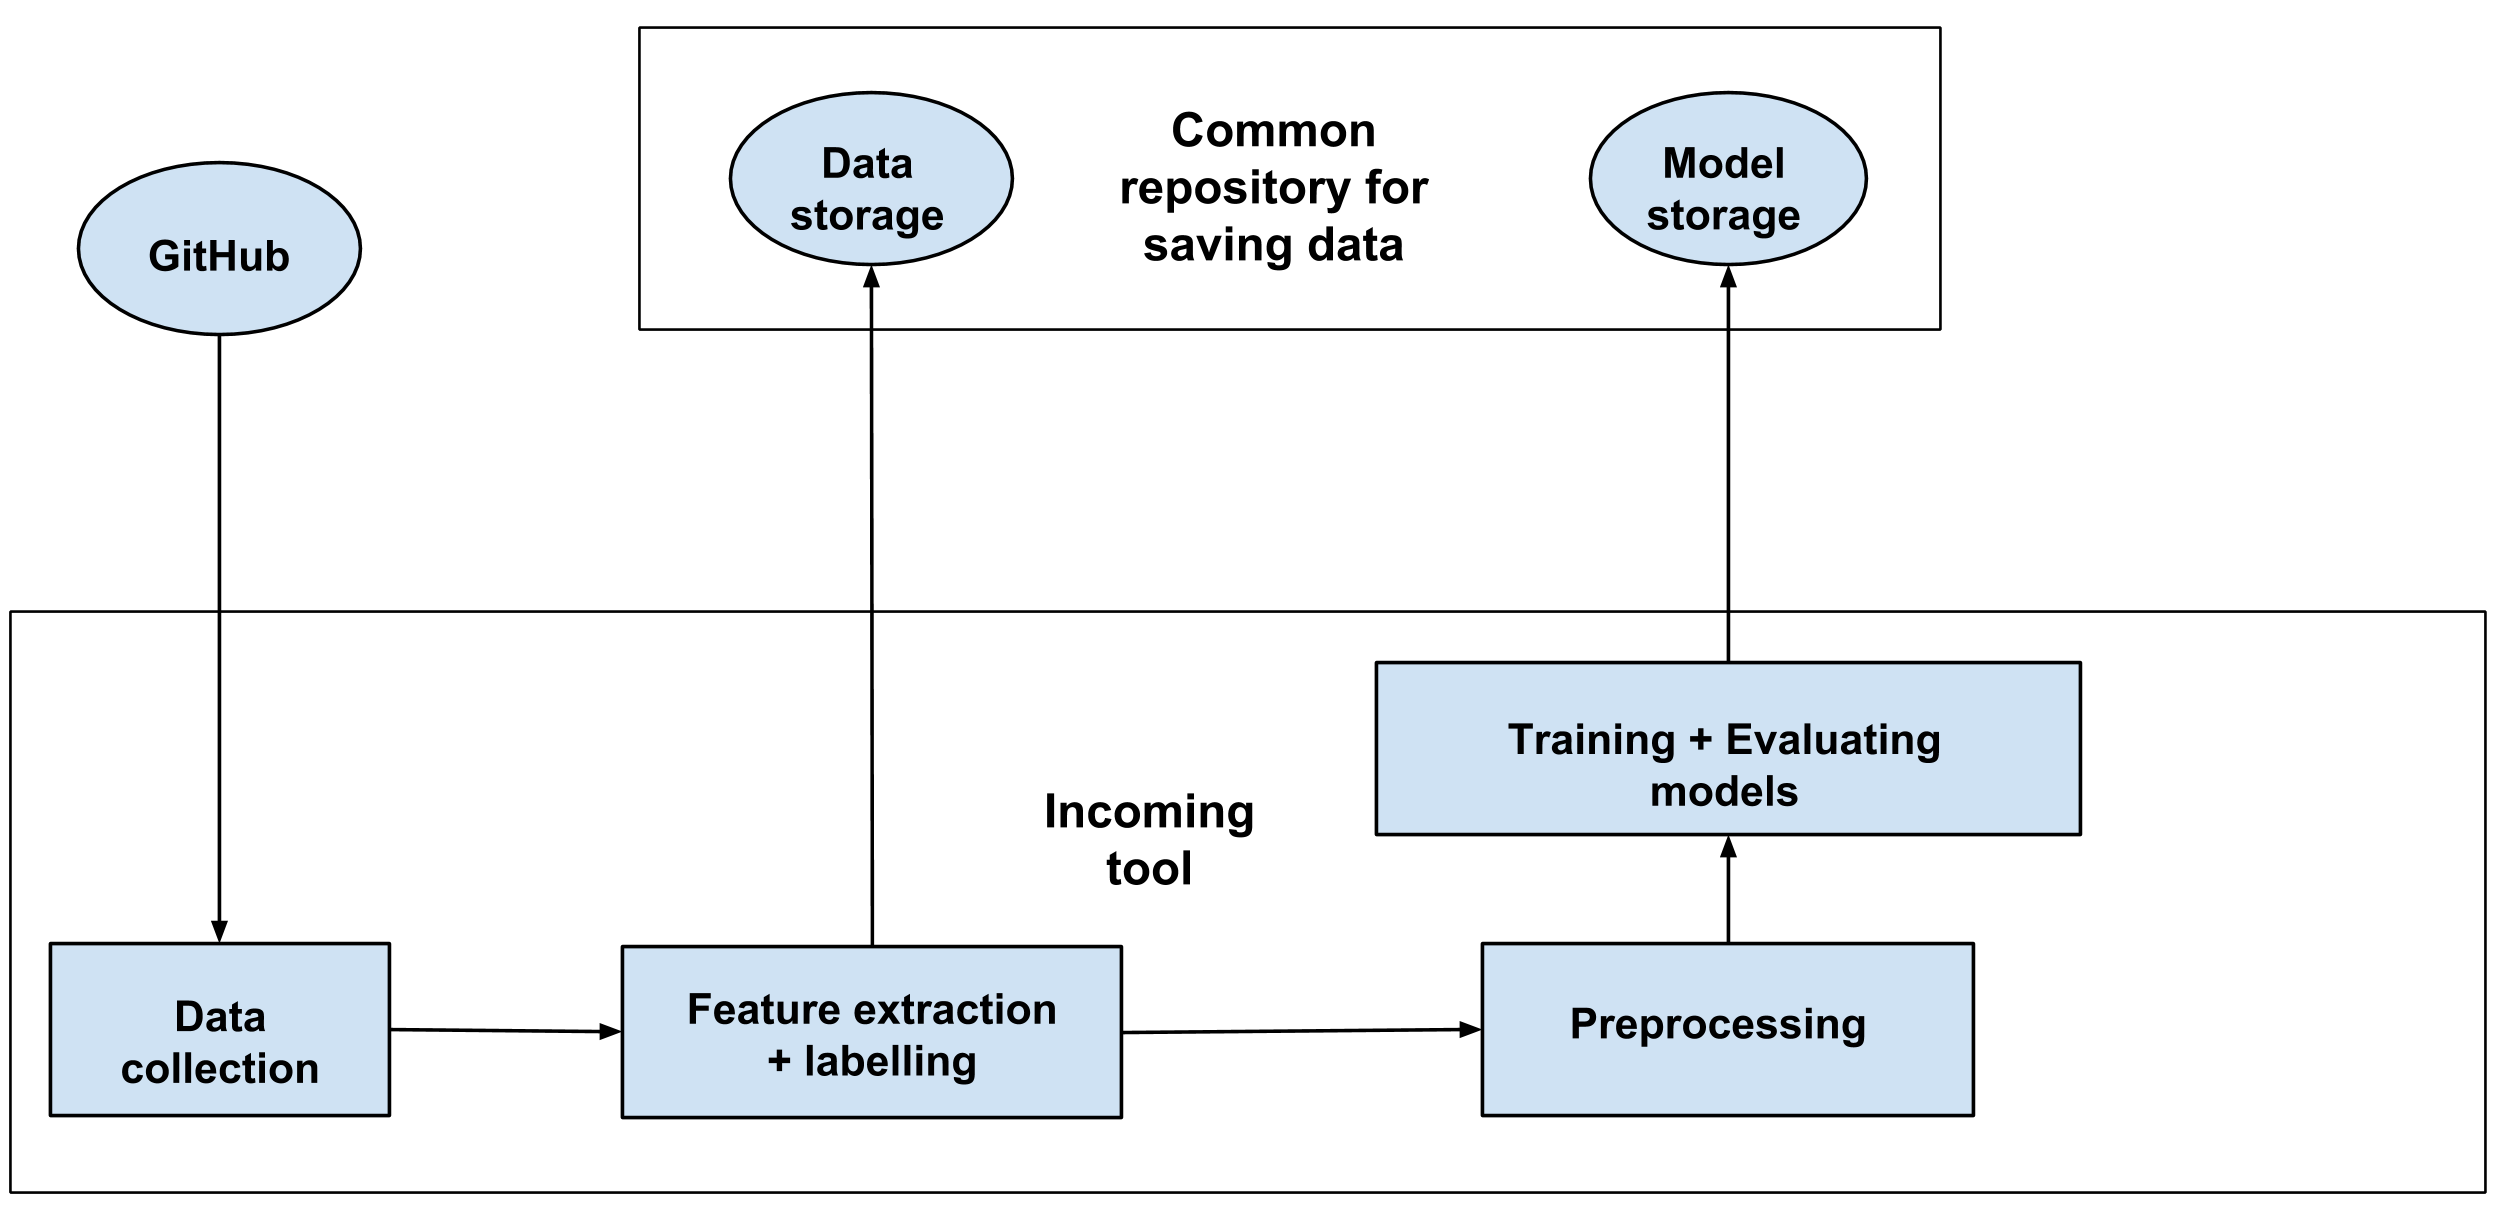
\includegraphics[width=1\textwidth]{images/Technical_Contribution/incoming_1.png}
\label{fig:incoming1}
\caption{Training mode}
\end{figure}


\section{Sending Predictions}

For the experiments, the tool was set up to send out predictions periodically to individual developers through Slack, a messaging tool. When making predictions, the tool would obtain a list of recent commits from several branches made by developers who registered to use the tool. Branches other than the master branch were included because development branches contain commits that are not reviewed during a pull request, hence the possibility of them being more risky. Once a prediction was made, it was sent to the author of the commit using messaging services such as Slack. 

Each prediction message sent on Slack would contain the link to the commit that was predicted on, the model's prediction for this commit (\textit{risky} or \textit{not risky}) as well as how confident the model was in that prediction. When machine learning models perform classification, they will output a probability for each class that an instance belongs to this class. The confidence is just the probability our commit is risky according to the model. The purpose of adding confidence to the message was because if a prediction had a 51\% confidence, this prediction would not be reliable as the chance of it being a false positive is very high. 

\begin{figure}[H]
\centering
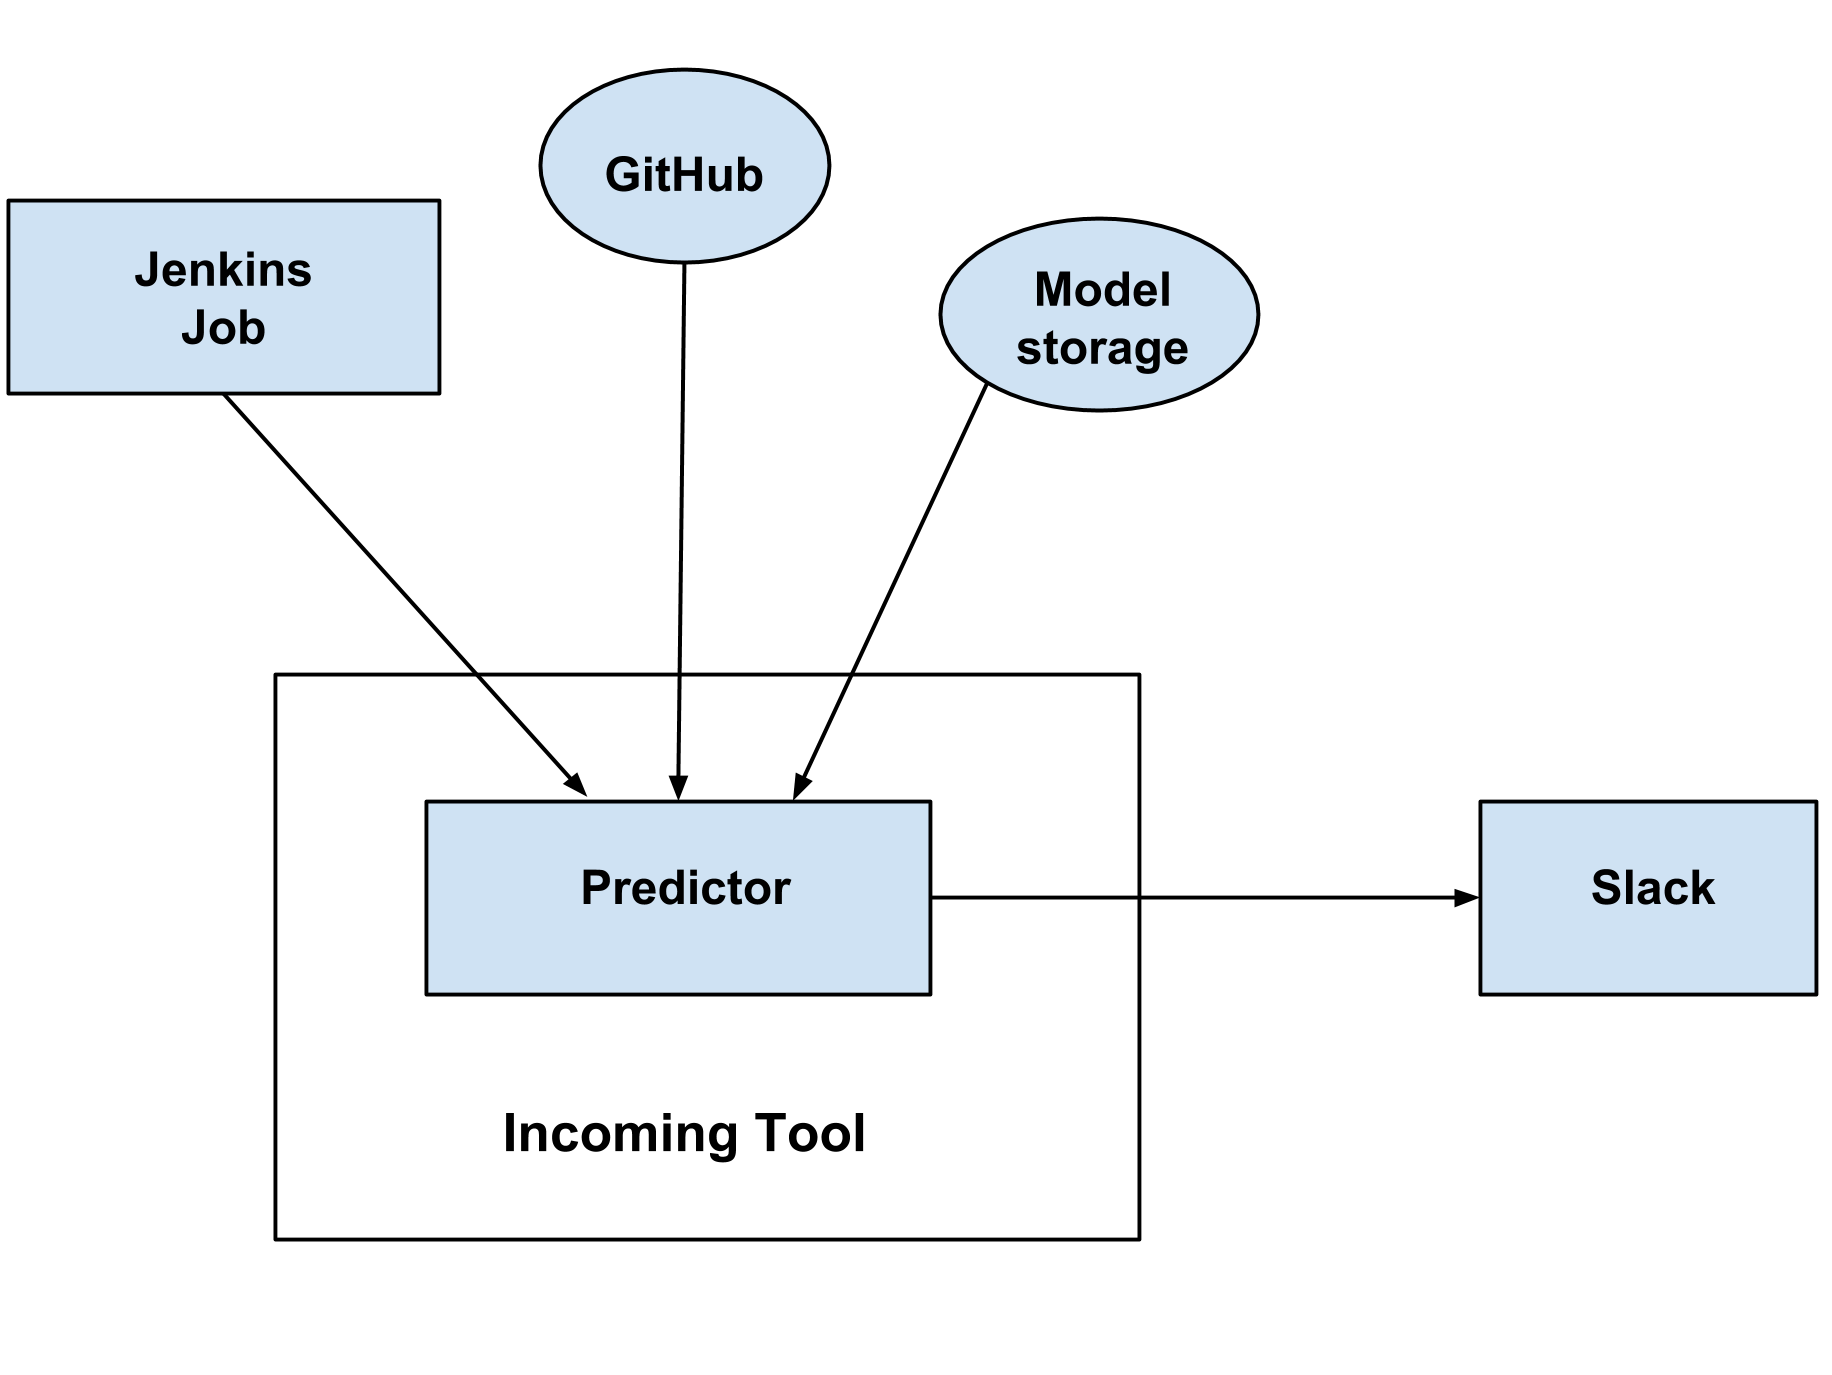
\includegraphics[scale=0.15]{images/Technical_Contribution/incoming_2.png}
\label{fig:incoming2}
\caption{Prediction mode}
\end{figure}

\section{Deployment}

In order to have data collection, training of models and predictions be performed frequently, the tool was deployed on King's continuous integration servers. The data collection and training was bundled into one Jenkins job whereas predictions ran in a separate job. These jobs were set up so that there were separate jobs for each project for which the tool was deployed too. Unlike the tool Commit Guru which analyzes commits once a user requests it, this tool runs autonomously. A proposed benefit of this would be that developers might be preoccupied with other tasks and forget to run the tool manually. Having it run in the background means that the tool can naturally be integrated into the developers' workflow. 

\end{document}